\subsection{Service Clients}\label{p:client}

This problem is designed to introduce the client-service structure. For this question you will be
using our implemented service and writing your own client to create a slightly different single
flower then before. See Figure~\ref{fig:2} for what the flower should look like.

The work for this problem should be done in file \texttt{client.py}.

\begin{figure}[h]
  \centering
  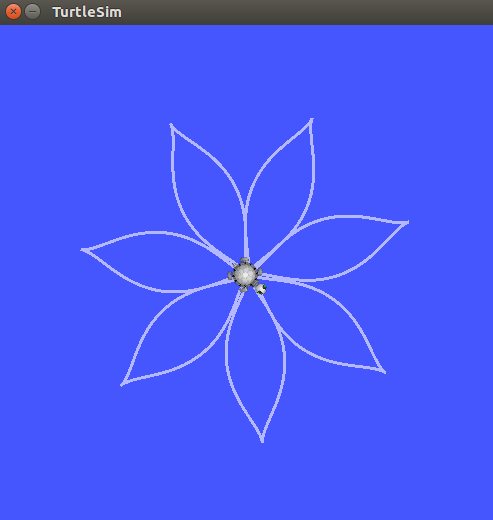
\includegraphics[width=150pt]{figures/p1/problem3.png}
  \caption{For Problem~\ref{p:client}. Service Clients}
  \label{fig:2}
\end{figure}

\begin{enumerate}[(a)]
  \item In \texttt{draw\_flower}:
  \begin{enumerate}[i.]
    \item Initialize your node with the name \texttt{drawing\_turtle}.
    \item Wait for the service \texttt{draw}.
  \end{enumerate}
  
  \item In \texttt{try} section: Fill in the service handle for the draw service with \texttt{draw}
  and \texttt{Draw}. Check \texttt{srv/Draw.srv} and \texttt{rospy} documentation for more information.

  \item After the \texttt{try} section: Fill in with a publisher that publishes to
  \texttt{/turtle1/cmd\_vel} with type \texttt{Twist} and queue size of 10 then set your rate to 5.

  \item In \texttt{while not rospy.is\_shutdown()} section:
  \begin{enumerate}[i.]
    \item Use the draw service to get the velocity message to publish. Look at
    \texttt{srv/Draw.srv} to determine the parameters and appropriate return name.
    \item Sleep for the previously stated rate.
  \end{enumerate}

  \item In \texttt{if \_\_name\_\_ == `\_\_main\_\_'}: Call your function to draw the flower!

  \item In \texttt{client.launch}:
  \begin{enumerate}[i.]
    \item Launch the turtlesim node.
    \item Launch the \texttt{draw\_service} node.
    \item  Launch the \texttt{draw\_flower} node.
  \end{enumerate}

\end{enumerate}



%%% Local Variables:
%%% mode: latex
%%% TeX-master: "../assessment"
%%% End:
